\documentclass[11pt, oneside]{article} 
\usepackage{geometry}
\geometry{letterpaper} 
\usepackage{graphicx}
	
\usepackage{amssymb}
\usepackage{amsmath}
\usepackage{parskip}
\usepackage{color}
\usepackage{hyperref}

\graphicspath{{/Users/telliott_admin/Dropbox/Tex/png/}}
% \begin{center} 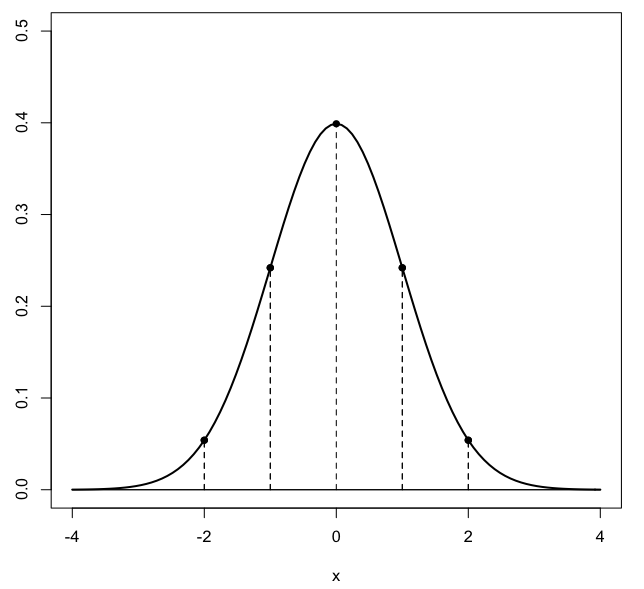
\includegraphics [scale=0.4] {gauss3.png} \end{center}

\title{GF(2)}
\date{}

\begin{document}
\maketitle
\Large

\subsection*{GF(2)}

Now we're getting closer to the main point.  We will be doing binary arithmetic and the coefficients of the polynomials come only from $0$ and $1$.  Therefore, the polynomials are of the form
\[ \sum_0^n x^n \] 

There are no coefficients now.  Either a term is zero or it is $x$ to some power like $x^n$.

GF(2) consists of the set \{0,1\}.

We define \textbf{addition}
\[ 0 + 0 = 0 \]
\[ 0 + 1 = 1 \]
\[ 1 + 0 = 1 \]
\[ 1 + 1 = 0 \]

Addition is the same as logical XOR.

\textbf{subtraction}
\[ 0 - 0 = 0 \]
\[ 1 - 0 = 1 \] 
\[ 0 - 1 = 1 \]
\[ 1 - 1 = 0 \]

Notice here that (i) $1 - 1 = 0$ because (from the first table) the arithmetic inverse of $1$ is just $1$ since $1 \oplus 1 = 0$, so $1 - 1 = 1 + 1 = 0$.  For a similar reason $0 - 1 = 1$.

Another reason is that in moving  $0$ to $-1$ we move by one unit.

\textbf{multiplication}
\[ 0 \times 0 = 0 \]
\[ 0 \times 1 = 0 \]
\[ 1 \times 0 = 0 \]
\[ 1 \times 1 = 1 \]

Multiplication is the same as logical AND.

\end{document}